
\chapter{量化质量管理} % Introduction chapter suppressed from the table of contents

如果我们相信Y理论,管理者的工作主要是提供资源,做好培训,订立更高的要求。

与一位有能力的开发组长对话:
你会听到他们都想把开发做好,确保开发质量,让客户满意。
他们也很清楚写好代码的原理,评审团员的代码,教他们如何学好公司的开发框架。
对也会每次冲刺后做复盘

\texttt{我问:很棒,请问你们过去质量有什么改进,生产率如何?}\\
\texttt{答:肯定有提升,但每个项目,每次迭代都不一样,无法比较}

让他们每次复盘回顾各个过程的缺陷排除率,
讨论制定下一个迭代的改进,便可以帮助团队往量化管理迈进第一步。

因为每一次迭代的挑战都不一样,
影响的因素也不同,无法只依赖公司依据历史项目数据,制定预测方程式,估计下一个迭代的缺陷范围(更不应把缺陷率当成考核指标),
只能依赖团队的分析与讨论制定下一个冲刺的缺陷目标。

前面``统计分析案例''便是基于 Y理论
的量化敏捷开发例子,以下是如何利用水晶球模型,降低验收系统缺陷的常见问题与解答;


\hypertarget{ux5982ux4f55ux5728ux8fedux4ee3ux56deux987eux4eceux7f3aux9677ux6570ux636eux5206ux6790ux5f97ux51faux9884ux6d4bux6a21ux578bux53c2ux6570}{%
\subsection{如何在迭代回顾从缺陷数据分析得出预测模型参数?}\label{ux5982ux4f55ux5728ux8fedux4ee3ux56deux987eux4eceux7f3aux9677ux6570ux636eux5206ux6790ux5f97ux51faux9884ux6d4bux6a21ux578bux53c2ux6570}}

提高阶段缺陷排除率,来完善软件交付时的质量,软件工程从60年代开始,起初主要用于瀑布式项目:


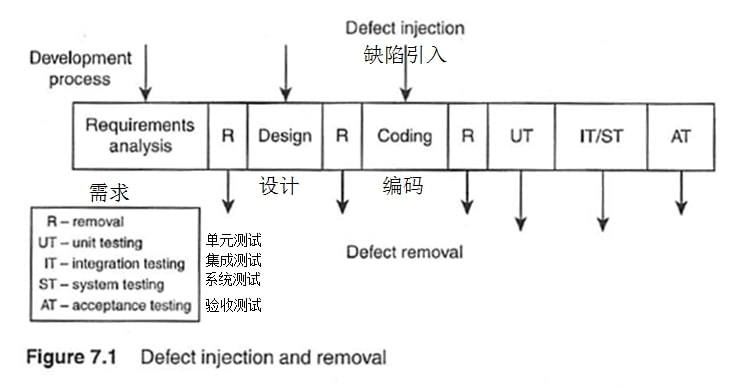
\includegraphics[width=10cm]{Jalote_emm_7_1_1_0.jpg}

Figure7.1,从需求到设计、编码、单元测试、系统测试、验收,整个开发过程大家都很熟悉,需求、设计、编码后都会评审来排除缺陷,但仅按这个流程不一定能确保质量。因为最终验收缺陷数取决于每个步骤排除当前缺陷的效率。下面我们介绍一下怎么从引进量化管理来提高开发质量:\\
\#要设定量化目标。例如希望最终遗漏到验收发现的缺陷数降多少?

\begin{enumerate}
\tightlist
\item
  也要设定中间阶段目标缺陷数,从而预测能否达到最终目标,不要等到最后才知道不满足
\end{enumerate}

可用缺陷排除率(Defect Removal Efficiency DRE) 来判断每一个过程的质量:\\

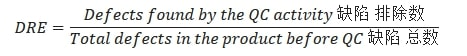
\includegraphics[width=10cm]{Ma3_1_0.jpg}

如果要最终质量好,缺陷排除率就要高。但计算缺陷排除率,必须要等到整个开发完成才可以计算,我们可以建立一个预测模型,模拟这个过程:\\
需求会引入缺陷,然后需求评审排除缺陷等等。利用蒙地卡罗预测模型估计每个阶段的缺陷数量。

Table 7.2 Defect Distribution in Infosys's PCB Infosys PCB的缺陷分布

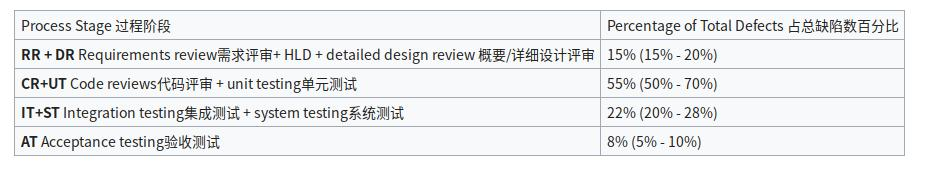
\includegraphics[width=10cm]{Screenshotfrom2022-01-23-2.jpg}


如果我们按上面 infosys
公司的各阶段缺陷利率百分比,设计与需求排除缺陷15\%,代码评审与单元测试55\%,集成/系统测试22\%,验收测试8\%,算出各阶段的缺陷输入与缺陷排除率,把参数输入蒙地卡罗预测模型:
表D1:\\

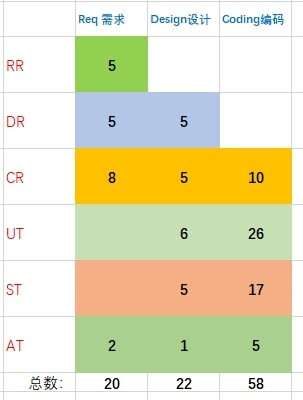
\includegraphics[width=10cm]{1113correctEgScreenshot_2021-11-13_212414.jpg}

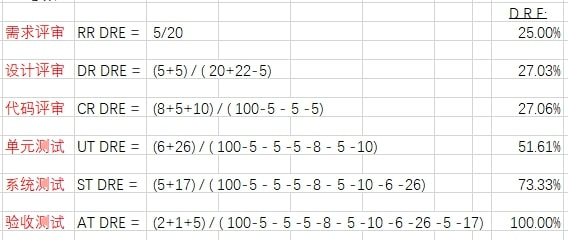
\includegraphics[width=10cm]{1113corrDreScreenshot_2021-11-13_212509.jpg}
得出下面Figure7.2,缺陷分布是中间最高头尾低,右面与左面不同,有条长尾巴,类似估算软件开发项目工作量的
Raleigh 曲线。

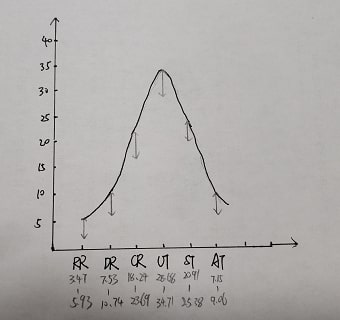
\includegraphics[width=10cm]{微信截图_20220107124057.jpg}


\includegraphics[width=10cm]{jalote_emm_7_2.jpg}

模型假定每个阶段的缺陷排除率都比较稳定,在某个范围之内,不同阶段引入的缺陷也在一定范围之内。
蒙地卡罗模型让我们可以设定缺陷排除率和缺陷输入数量的波动范围,预测各阶段缺陷排除分布范围(不仅仅看单点数)。

\hypertarget{ux56e2ux961fux5df2ux7ecfux6309ux654fux6377ux8fedux4ee3ux5f00ux53d1ux60f3ux91cfux5316ux7ba1ux7406ux4e0dux77e5ux5e94ux5982ux4f55ux5f00ux59cb}{%
\subsection{团队已经按敏捷迭代开发,想量化管理,不知应如何开始}\label{ux56e2ux961fux5df2ux7ecfux6309ux654fux6377ux8fedux4ee3ux5f00ux53d1ux60f3ux91cfux5316ux7ba1ux7406ux4e0dux77e5ux5e94ux5982ux4f55ux5f00ux59cb}}

很多人都误解度量分析必须像大数据分析一样,要有大量数据,用很多因子来求出一个漂亮的方程式,才算成功。其实是反过来,如果像要收集的数据量越大,变量越多,量化过程改进越难成功,开发人员越抵触。所以我们必须要针对想改进的重点收集对应数据。

\framebox{%
\begin{minipage}[t]{0.97\columnwidth}\raggedright
{如何建立并完善缺陷预测模型的例子}
公司度量分析人员展示了一个大表,上面有五、六十个项目变量,包括缺陷、进度、工作量等等,密密麻麻几十个变量。\\
{我问}:为什么你们要收集这么多数据量?你们的改进目标是什么?\\
{度量分析人员说}:我们要提高生产率、减少进度偏差,也要降低最终的客户的缺陷密度。\\
{我}:我们可参考''MA2统计分析案例``,靠尽早发现缺陷,加强前面的评审效率来减少遗漏到后面的缺陷,减少返工。如果大家都相信这可行,就应该专注这模型相关的度量。如进度偏差、生产力、质量都要做好,反而就没有针对性,量化过程改进更难成功。如果能尽早发现缺陷并修复,后面返工量便可倍数降低,生产力自然会提升。\\
我们看看这预测缺陷模型,比如你们有什么不同的评审方式?效果有什么不同?\\
{答}:我们跟开发讨论过,确实有些区分,例如,如果我们在前期有做正式评审,质量都会好一些,但是如果没有的话,后面确实缺陷就多了。如果我们有明确需求,例如按活动、实体方式明确写出来,跟没有的话也会有质量的区分。有些项目有规定要静态扫描代码并记录缺陷,后期的缺陷数会较少。\\
{我}:所以如果你可以估计各种方式的缺陷排除率/引入缺陷率,便可使用模型预测最终会遗漏多少缺陷。
它就是一个项目经理可利用这蒙地卡罗预测工具,帮你去比较各种方法,制定缺陷数目标。但开始时缺乏数据,先参考行业数据估一下数,同时也做一些实验,看看不同的组合,看看对缺陷率,缺陷排除率和工作量等有什么影响。\\
例如有些团队利用静态代码扫描预先找出代码缺陷,就可以做个实验,区分一下是否代码扫描的话后面的缺陷会减少,排除缺陷的百分利是多少?\\ 开始的时候可能数据量不多,一两个项目,慢慢项目多了数据也可以看是否稳定,开始变成团队,甚至公司的基线。所以开始时不要太计较准不准,而是尽快利用这概念开始量化。\\
小时候看病,中医是用望闻问切的方式;西医就是用听诊器听心跳、呼吸,看舌头、口腔,然后也是听你的问题描述,便可以诊断开药了。现在去医院排队看病,医生第一件事就给你开四五张各类的检查单,通过这些检查报告做诊断。虽然我是外行,但我觉得小时候那种不超过十分钟诊断过程不会比现代的起码两个小时的诊断质量差。\\
{经验教训}:度量与分析同理,我们只要针对最相关的度量数据(也容易收集到)来诊断,才有效,还省钱。\strut
\end{minipage}}

\hypertarget{ux6c34ux6676ux7403ux5de5ux5177ux5e26ux6765ux4ec0ux4e48ux4ef7ux503cux53efux4e0dux53efux4ee5ux4e0dux7528ux5b83}{%
\subsection{水晶球工具带来什么价值,可不可以不用它?}\label{ux6c34ux6676ux7403ux5de5ux5177ux5e26ux6765ux4ec0ux4e48ux4ef7ux503cux53efux4e0dux53efux4ee5ux4e0dux7528ux5b83}}

例如我们有10个步骤。 如果每步都估算天数,10个步骤的 总天数就是500天
(把10个估算值加起来)。

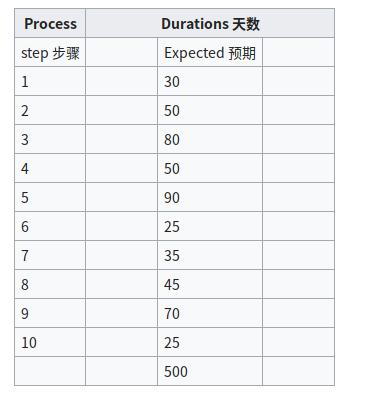
\includegraphics[width=10cm]{Screenshotfrom2022-01-23-3.jpg}


但如果每个步骤都是3点估算 - 加上最短和最长天数, 便不能直接加起来。

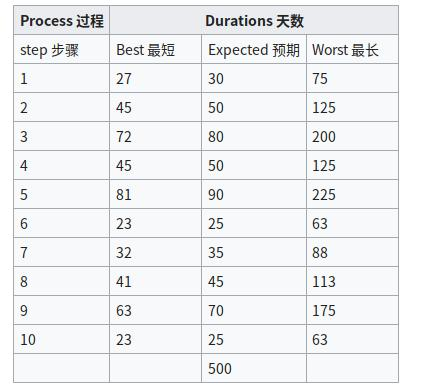
\includegraphics[width=10cm]{Screenshotfrom2022-01-23-4.jpg}

这例子很明显看到每一步最长的估算都偏高,所以可预计总天数应不止500天,
但估多少才合适?

水晶球工具原理:按每步骤的三点估算随机估一个数,然后把十步骤的随机估算值加起来得出总数;假如重复五千次,便可得出下面的分布:


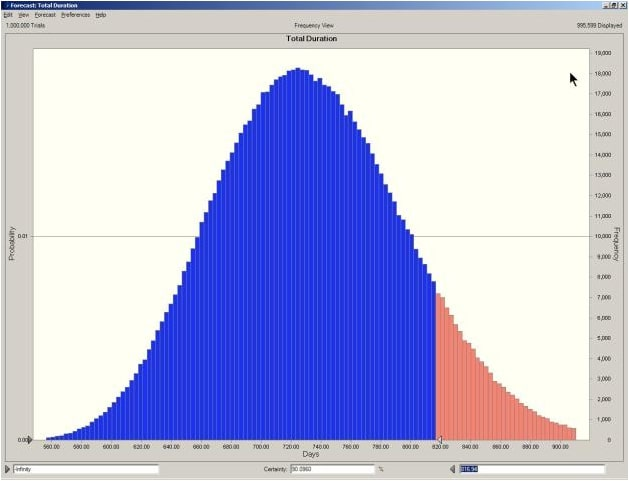
\includegraphics[width=10cm]{HMTT_v1_3_s77.jpg}

预计总天数在817天内的概率是90\%,500天内的机会非常低。
所以工具可以帮我们简单估计范围。

\hypertarget{ux5982ux4f55ux5229ux7528ux9884ux6d4bux6a21ux578bux5e2eux6211ux4eecux9884ux8ba1ux6bcfux4e2aux8fc7ux7a0bux7684ux7f3aux9677ux8303ux56f4}{%
\subsection{如何利用预测模型帮我们预计每个过程的缺陷范围?}\label{ux5982ux4f55ux5229ux7528ux9884ux6d4bux6a21ux578bux5e2eux6211ux4eecux9884ux8ba1ux6bcfux4e2aux8fc7ux7a0bux7684ux7f3aux9677ux8303ux56f4}}

如果没有预测模型,也可以按以往项目的缺陷数估计新项目的阶段缺陷数范围。例如,以表7.3的例子,ABC项目已经做过两轮,收集了工作量,验收和系统测试缺陷数据如下:

Table 7.3 Past Projects Data for Example 1 过去项目数据

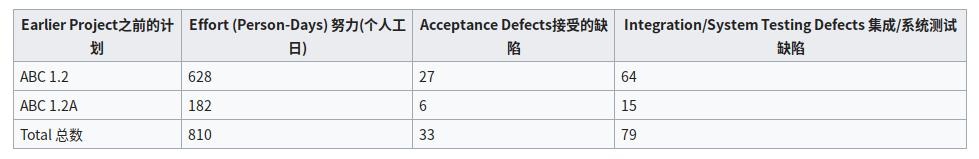
\includegraphics[width=10cm]{Screenshotfrom2022-01-23-5.jpg}

因为新的ABC项目开发,在语言、项目类型、客户业务等都很类似,所以我们可以依据以往两次项目估计新项目的缺陷范围。如果我们估计新一期的项目的工作量是1519人天,我们就可以按验收测试的总数33得出新项目的缺陷数是62。也可以从历史数据估计缺陷数是45,因为45低于62,最后我们就定验收缺陷目标是45到60之间。如果我们按照以前的项目建立预测模型,首先可以输入来是功能点数,看看实际的验收缺陷数和系统测试缺陷数是否在预测范围之内。把新项目的功能点数输入预测模型,便可以得出验收缺陷的范围。同样我们也可以不利用预测模型,从以往两个项目的缺陷数按比例估算出系统测试和集成测试总共的缺陷数是148。我们也可以同样得出系统测试的范围,目标范围是148到180缺陷之间。所以如果我们一直有收集预测模型,就可以直接得出每个阶段缺陷范围预估。

\hypertarget{ux4e00ux76f4ux6709ux505aux8fedux4ee3ux56deux987eux4f46ux7f3aux4e4fux91cfux5316ux5206ux6790ux5e94ux5982ux4f55ux5f00ux59cb}{%
\subsection{一直有做迭代回顾,但缺乏量化分析,应如何开始?}\label{ux4e00ux76f4ux6709ux505aux8fedux4ee3ux56deux987eux4f46ux7f3aux4e4fux91cfux5316ux5206ux6790ux5e94ux5982ux4f55ux5f00ux59cb}}

改变习惯最难,要从定性升到定量管理必须先让团队了解为什么要数据,有什么用;也让大家从团队数据自己找出不足。下面是一天培训安排:\\

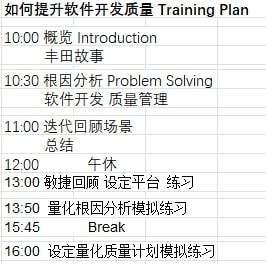
\includegraphics[width=10cm]{TraininPlanScreenshot_2021-11-24_210344.jpg}

上午我们介绍了过程改进,根因分析,和质量成本(Cost of
Quality)等概念。我和3位组长大家做一个回顾的场景演示(十五分钟左右),介绍回顾的五个步骤,让他们感受一下迭代回顾应该怎么开始,怎么讨论,怎么分析数据并结论:\\
\#Set the stage 设置舞台

\begin{enumerate}
\tightlist
\item
  Gather Data 收集数据
\item
  Generate Insights 分析,找出根因
\item
  Decide What to Do 决定后面做什么
\item
  Close the Retrospective 结束回顾
\end{enumerate}

下午一点钟大家吃完饭,必须动起来,所以我就选了两个设置舞台互动练习。例如,
Focus On/Focus Off:应与否小组互动练习:

\begin{description}
\item[]
\begin{description}
\tightlist
\item[]
调研 (Inquiry) vs 辩护(Advocacy)\\

对话 (Dialogue) vs 辩论 (Debate)\\

交流 (Conversation) vs 爭吵 (Argument)\\

理解 (Understanding) vs 防护(Defending)\\
\end{description}
\end{description}

让他们一组最多4人选最好的方式去表达上面左面词汇跟右面词汇的区分。目的是让大家理解在回顾讨论时,要有正确的心态,如对事不对人。他们有些用各种角色扮演什么是吵架,什么是交流,让观众和表演者更能感受到量化回顾先要有对事不对人的心态。

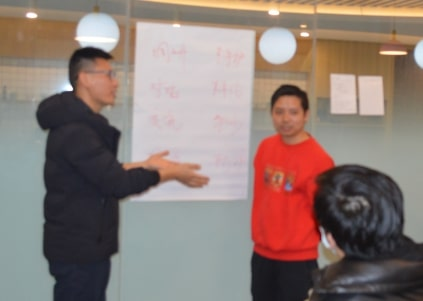
\includegraphics[width=6cm]{1498.jpg}
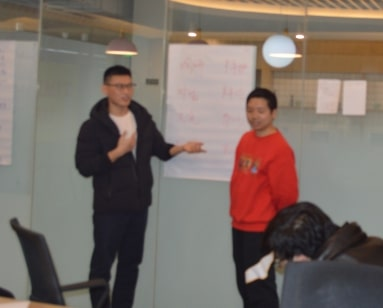
\includegraphics[width=6cm]{1499.jpg}

时间有限,第二个练习立马就要他们分析迭代缺陷数据。每组都收到:\\
*系统测试缺陷(打印出来)

\begin{itemize}
\tightlist
\item
  两位开发人员的迭代工时表记录了这个迭代他们花在系统测试bug修改和代码工作量与缺陷(评审缺陷)
\item
  一张需求/设计评审问题单
\item
  迭代缺陷分析表,类似上面 表D1
\end{itemize}

要求他们按自己分析那些原始数据。找出每个阶段的缺陷,并识别缺陷是源自需求,设计,还是代码,计算出每个阶段的缺陷排除率。然后把缺陷和排除率输进水晶球模型,估计每个阶段的缺陷范围。

从这第一轮迭代数据,从模型跑出来的个阶段缺陷预测范围,会看到模型只能预计现在的状态,系统测试的缺陷最多,验收其次
,其他都很少(团队的基线)然后也估计每个阶段的缺陷平均返工工作量。

\framebox{%
\begin{minipage}[t]{0.97\columnwidth}\raggedright
某团队互动练习例子\\
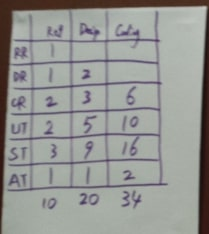
\includegraphics[width=8cm]{1reviewDefectsCountScreenshot_2021-12-01_211909.jpg}\\

\begin{itemize}
\tightlist
\item
  估算 各DRE
\end{itemize}

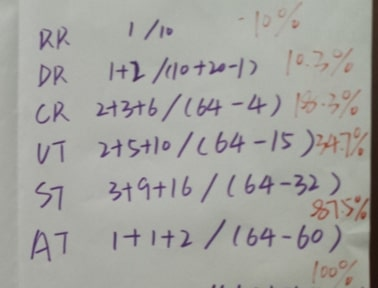
\includegraphics[width=8cm]{2DreEstimateScreenshot_2021-12-01_212049.jpg}\\
\begin{itemize}
\tightlist
\item
  从迭代缺陷数据与DRE,利用水晶球估计各缺陷范围,还是ST缺陷居多
\end{itemize}

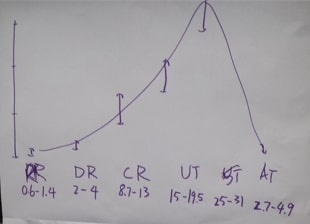
\includegraphics[width=8cm]{2AxtalBallPredictScreenshot_2021-12-01_212455.jpg}\\

\begin{itemize}
\tightlist
\item
  从各过程缺陷数与总返工工作量,估计缺陷返工工作量
\end{itemize}

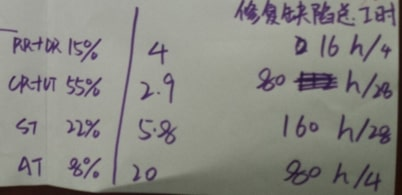
\includegraphics[width=8cm]{4reworkByPhaseScreenshot_2021-12-01_214838.jpg}
\strut
\end{minipage}}


我解读:``因为你们本来缺陷都是后期才被发现,所以模型的排除率分析也只能反应现状,还是系统测试问题最多。我们也看到,你们每个阶段的缺陷返工工作量是多少?确实验收缺陷返工工作量最大;系统缺陷第二。''\\
我接着说:''如果可以把缺陷预先发现,是否可以减少总工作量,提高效率?''\\
第三个练习:要求他们接着用头脑风暴K-J方式和帕累托图,分析缺陷到系统测试才被发现的原因。针对根本原因在下一个迭代采取改进措施,并估计下一个迭代的缺陷分布,重新计算排除率,再利用预测模型估计每个阶段的缺陷数范围。今次预测便应是大部分缺陷在编码阶段或之前被发现。


\includegraphics[width=10cm]{xt2_1.jpg}
%\includegraphics[width=6cm]{t_3.jpg}

如果我们没有这些数据分析,只能泛泛的提想法、意见,没有像现在这么具体从数据识别出一些针对性的解决方法,也因为现在每个阶段的缺陷有范围有数,我们后面做评审时,便有目标,不会只是走评审过程。

团队在开始从定性到定量管理的时候,可以在回顾时,用这个练习的思路,分析一下刚刚迭代的缺陷排除率和缺陷引入,以前没有这种细化的数据,根因分析可能只看到系统测试缺陷的总数多少,用了这个排除率的分解,就可以让团队了解主要问题来自哪里,针对性分析根因和对应措施。例如发现大部分的缺陷来自代码,就深入地去看代码出了什么问题,那一类代码缺陷比较多,针对这一类的缺陷讨论原因,下一轮做对应改进措施,并制定新一轮的量化目标。\\
量化回顾也让团队成员了解到自己的问题,更了解自己的质量和水平。

团队基于练习2的数据,计划利用高保真原型方式,提高需求设计阶段发现缺陷的比例,希望把缺陷发现阶段前移:


\framebox{%
\begin{minipage}[t]{0.97\columnwidth}\raggedright
团队基于数据,计划利用高保真原型方式,提高需求设计阶段发现缺陷的比例,希望把缺陷发现阶段前移

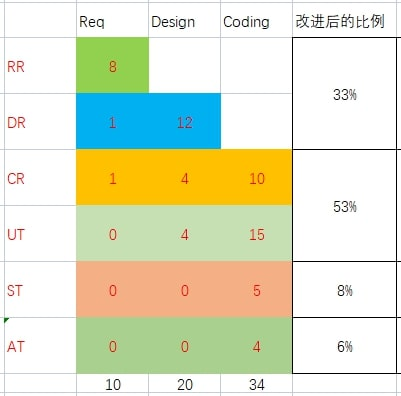
\includegraphics[width=8cm]{微信截图_20211221134318.jpg}

也计算每个阶段的缺陷排除率

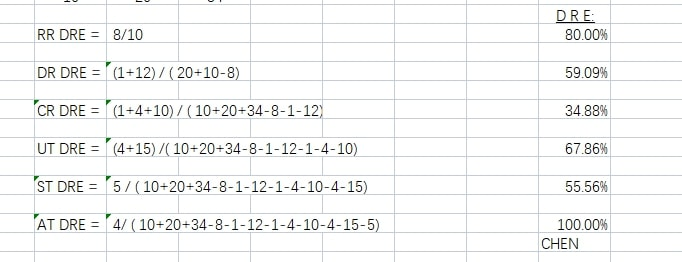
\includegraphics[width=8cm]{微信截图_20211207131759.jpg}

最后画出来的曲线图

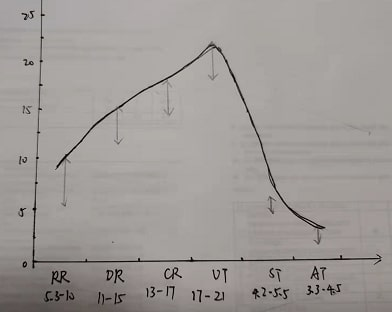
\includegraphics[width=8cm]{微信截图_20211207132712.jpg}

把缺陷发现的高峰从系统测试迁移到单元测试,系统测试的缺陷数5个左右。\strut
\end{minipage}}

\hypertarget{ux5982ux679cux6211ux4eecux662fux4e00ux4e2aux5168ux65b0ux9879ux76eeux6ca1ux6709ux50cfabcux90a3ux79cdux6709ux5386ux53f2ux6570ux636eux53c2ux8003ux662fux5426ux5c31ux7528ux4e0dux4e86ux9884ux6d4bux6a21ux578bux5462}{%
\subsection{如果我们是一个全新项目,没有像ABC那种有历史数据参考,是否就用不了预测模型呢?}\label{ux5982ux679cux6211ux4eecux662fux4e00ux4e2aux5168ux65b0ux9879ux76eeux6ca1ux6709ux50cfabcux90a3ux79cdux6709ux5386ux53f2ux6570ux636eux53c2ux8003ux662fux5426ux5c31ux7528ux4e0dux4e86ux9884ux6d4bux6a21ux578bux5462}}

其实反过来,预测模型的目的是帮我们更好去试一些新的做法,帮我们估计如果某些过程可以降低缺陷数的输入,或者提高缺陷的排除率,最终会有什么效果,而不是仅仅依赖以往项目历史数据,预测缺陷范围,例如:

Table 7.5 Project Quality Goals of the WAR Project
WAR项目的项目质量目标\\
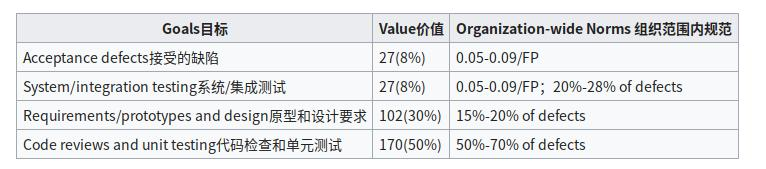
\includegraphics[width=10cm]{Screenshotfrom2022-01-23-8.jpg}


这个WAR
项目,用了新的技术和工具,以前没有类似项目。但我们估计缺陷的引入还是不变,差不多每一个功能点一个缺陷。所以这个项目新项目我们估计总共的缺陷数大概为340。我们估计因为会用原型法和新的评估方法,会大大提高需求与设计阶段的缺陷排除率,从而估计系统测试缺陷率和验收测试的缺陷率会降低。本来如果没有预测模型的话,我们只能主观估计百分比会降低,但有了预测模型,我们确实可以尝试改变参数,看能否估计缺陷分布的变化,也帮我们验证这假定是否可行。最终我们验证了确实这个百分比是可行。如果没有预测模型便难以做到。

上面练习二练习三两者前后比较便是一个实例:\\

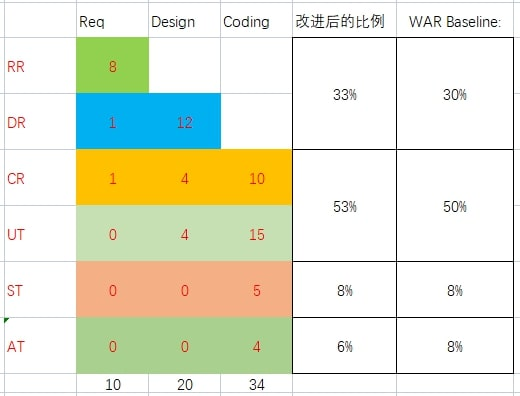
\includegraphics[width=10cm]{微信截图_20211221134353.jpg}

例如上图看到练习三的缺陷比例比WAR 的要求稍微高一些。

\hypertarget{ux5982ux4f55ux6709ux6548ux6536ux96c6ux7f3aux9677ux76f8ux5173ux6570ux636eux5206ux6790ux5982ux4f55ux6539ux5584ux8d28ux91cf}{%
\subsection{如何有效收集缺陷相关数据,分析如何改善质量}\label{ux5982ux4f55ux6709ux6548ux6536ux96c6ux7f3aux9677ux76f8ux5173ux6570ux636eux5206ux6790ux5982ux4f55ux6539ux5584ux8d28ux91cf}}

最有效的方式就是每次迭代两周回顾时,同时看看本迭代缺陷的相关数据。如果每天去看太费劲。如果一个瀑布项目,最终结束才回顾,三四个月,大家可能都忘记。以刚才这个例子,如果他们每个人都统计了代码的缺陷数和工作量,迭代回顾时,便可以列出系统测试缺陷总数。然后分析一下那些是源自需求,那些源自设计,那些源自代码。同样也可以对代码评审的问题做分析,综合起来就可以估算今次迭代,需求的评审缺陷排除效率、设计评审缺陷排除效率、代码评审缺陷排除效率。
数据分析最终目的是帮我们团队可以从数据洞察问题所在,给反馈,让他们知道弱在哪里,哪方面需要完善。回顾反馈后,就可以立马在下一个迭代做改进。虽然自动化系统的支持很重要,但也不能单靠系统。有些企业,设备、支撑、平台都很齐全、很自动化,可能系统也里面有很多要用的数据,但当我问他们过去半年,哪方面有具体的改进,与相关数据?但因为他们没有从针对改进目标来收集数据,这些基本的问题就答不出来。所以有些人说要在职场里面晋升,必须要从老板的视角看事情。所以如果你做了很多自动化流程,但不能解答老板问你过去半年质量改好多少、生产率是否要提升等基本问题,就很难得到高层对你过程改进的持续支持。

\hypertarget{ux5982ux4f55ux6536ux96c6ux5355ux5143ux6d4bux8bd5ux7f3aux9677---ux5f88ux5c11ux4ebaux4f1aux81eaux5df1ux6d4bux4e86ux53c8ux7ed9ux81eaux5df1ux8bb0ux5f55ux7f3aux9677ux57faux672cux90fdux662fux53d1ux73b0ux7f3aux9677ux76f4ux63a5ux5c31ux4feeux590dux4e86ux81eaux52a8ux5316ux5355ux5143ux4e5fux662fux4e0dux4f1aux8bb0ux5f55ux7f3aux9677ux76f4ux63a5ux5c31ux81eaux5df1ux89e3ux51b3ux4e86ux4e0dux4f1aux518dux8bb0ux5f55ux7f3aux9677-ux5982ux4f55ux53efux4ee5ux7b80ux5355ux6709ux6548ux7684ux6536ux96c6ux7f16ux7801ux7f3aux9677ux4e0eux8fd4ux5de5ux5de5ux4f5cux91cfux6570ux636e}{%
\subsection{如何收集单元测试缺陷 -
很少人会自己测了又给自己记录缺陷,基本都是发现缺陷直接就修复了,自动化单元也是不会记录缺陷,直接就自己解决了,不会再记录缺陷。
如何可以简单、有效的收集编码缺陷与返工工作量数据?}\label{ux5982ux4f55ux6536ux96c6ux5355ux5143ux6d4bux8bd5ux7f3aux9677---ux5f88ux5c11ux4ebaux4f1aux81eaux5df1ux6d4bux4e86ux53c8ux7ed9ux81eaux5df1ux8bb0ux5f55ux7f3aux9677ux57faux672cux90fdux662fux53d1ux73b0ux7f3aux9677ux76f4ux63a5ux5c31ux4feeux590dux4e86ux81eaux52a8ux5316ux5355ux5143ux4e5fux662fux4e0dux4f1aux8bb0ux5f55ux7f3aux9677ux76f4ux63a5ux5c31ux81eaux5df1ux89e3ux51b3ux4e86ux4e0dux4f1aux518dux8bb0ux5f55ux7f3aux9677-ux5982ux4f55ux53efux4ee5ux7b80ux5355ux6709ux6548ux7684ux6536ux96c6ux7f16ux7801ux7f3aux9677ux4e0eux8fd4ux5de5ux5de5ux4f5cux91cfux6570ux636e}}

很多团队说"我们都有评审代码,但问题都直接改正了,没有记录。``\\
后面便不知道有多少缺陷,无法量化分析。如果要求开发人员按系统测试缺陷记录方式,在缺陷管理系统里面一条一条记,大家会觉得太花时间不愿意做。
可以利用工具帮助,例如可利用GIT做代码评审记录,也可以在GIT系统里面跟踪评审问题。不需要把问题另外记在系统测试缺陷跟踪系统,但每条问题在GIT系统里都有痕迹。开发就可以从中数出大概共有多少代码评审缺陷。如果平常也记录了每天所花的时间,他用来修改bug的工作量也有统计数据了。\\
建议可以考虑我在《个人写程序》案例分享的做法一样,要求每人自己每天记录当天工时花在什么地方?比如花在缺陷的修复的是多少,迭代结束回顾时,每人看看自己的记录。团队迭代回顾时,因为在系统里面也有评审缺陷的跟踪也可以数出来缺陷是多少,从而可以算到平均一个缺陷花多少返工工时。这样就不会要开发人员花太多时间做记录,但回顾还可以收集到开发过程的所需数据。

例如,互动练习时,要学员利用开发人员工时表
(模拟他们迭代中用于改缺陷的工时,与评审缺陷数,与开发和修正代码的工时):

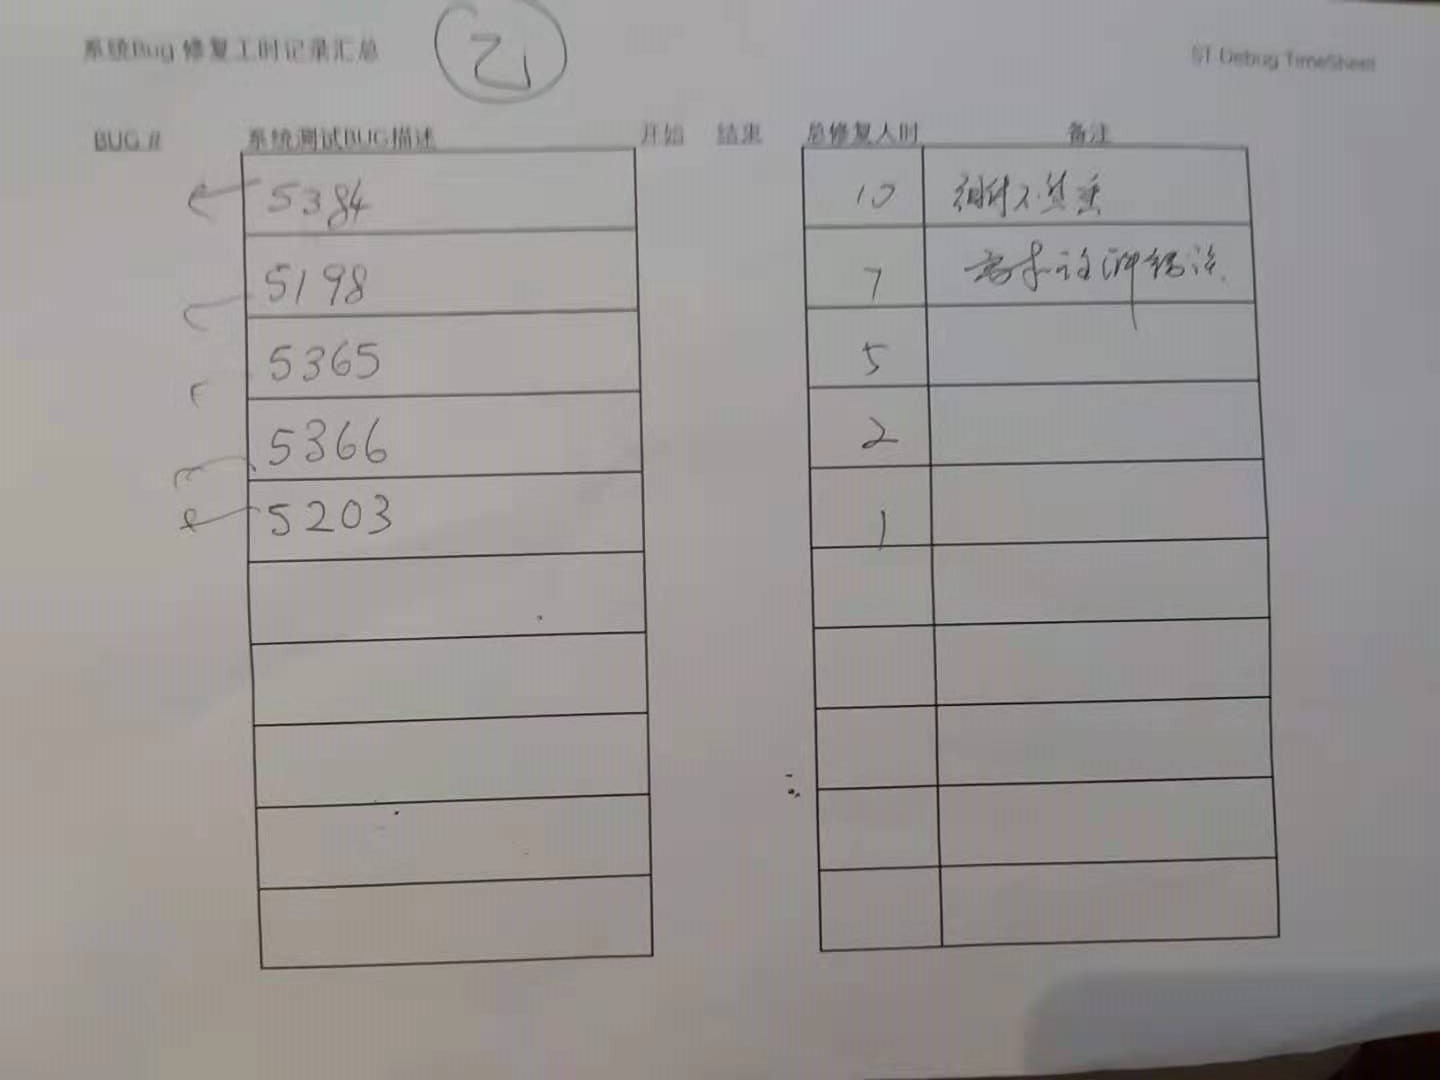
\includegraphics[width=10cm]{缺陷表4.jpg}


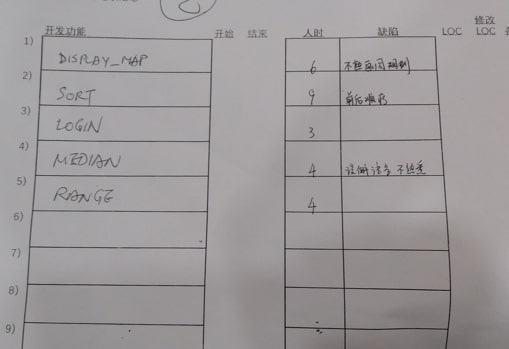
\includegraphics[width=10cm]{微信截图_20211228095232.jpg}

\hypertarget{ux6211ux4eecux505aux91cfux5316ux7ba1ux7406ux8981ux6536ux96c6ux591aux5c11ux6570ux636eux624dux591f}{%
\subsection{我们做量化管理,要收集多少数据才够?}\label{ux6211ux4eecux505aux91cfux5316ux7ba1ux7406ux8981ux6536ux96c6ux591aux5c11ux6570ux636eux624dux591f}}

你的问题问的不对,你可以想象每个公司开始的时候都没有什么数据,都是先试点开始,数据很少。如果我必须要多少数据才可以做量化,公司永远启动不了量化管理。所以还是先试点一、两个项目,看结果效果才进一步推广扩大。所以开始的时候数据不多,这用不上统计分析的那些方程式和假设检验那些数,正如我们在MA1分享文章里面那些例子,你简单把那些数画出来就可以了,看看是否第一个、第二个项目不同迭代的数是否很分散还是比较集中?如果都是很散的话,项目首先应该是想为什么这么理想?比较集中稳定下来才算才值得定制性。你定一个很宽的基线,用途不大。就好比你跑步,有时候一公里跑很快:六分钟,但有些时候可能要九甚至十分钟你应先探探索差异的原因,这么宽的基线没有什么参考作用。

\hypertarget{ux8fd9ux4e2aux7f3aux9677ux9884ux6d4bux6a21ux578bux662fux5426ux4ec5ux9002ux7528ux4e8eux7011ux5e03ux5f0fux5f00ux53d1ux6a21ux578b-ux5982ux679cux6211ux4eecux7528ux8fedux4ee3ux654fux6377ux662fux5426ux4e0dux9002ux7528}{%
\subsection{这个缺陷预测模型,是否仅适用于瀑布式开发模型?
如果我们用迭代/敏捷是否不适用?}\label{ux8fd9ux4e2aux7f3aux9677ux9884ux6d4bux6a21ux578bux662fux5426ux4ec5ux9002ux7528ux4e8eux7011ux5e03ux5f0fux5f00ux53d1ux6a21ux578b-ux5982ux679cux6211ux4eecux7528ux8fedux4ee3ux654fux6377ux662fux5426ux4e0dux9002ux7528}}

我本来从美国SEI学这个蒙地卡罗模型时,我也以为它只适用于瀑布开发。但其实我们也可以把它用于迭代开发中。把每个迭代(或冲刺)看成了一个两周的小瀑布,每次回顾会时,收集本次迭代各种评审与测试缺陷数,与预测值比较,\\
在瀑布开发,我们用模型来预测每个阶段的缺陷范围,确保最终能达到系统/验收测试缺陷目标。
在迭代回顾会,我们用预测模型来分析哪些过程的缺陷排除效率低,识别改进方向,
在下一个迭代尝试一些新方法,希望能改善质量。
也可以用模型来预估如果能提升某评审环节的缺陷排除效率,能提高评审的发现缺陷数多少,能减少系统测试缺陷多少?

\hypertarget{ux8fd9ux65b9ux6cd5ux5982ux4f55ux5e2eux56e2ux961fux6ee1ux8db3cmmiux9ad8ux6210ux719fux5ea6ux8981ux6c42}{%
\subsection{这方法如何帮团队满足CMMI高成熟度要求?}\label{ux8fd9ux65b9ux6cd5ux5982ux4f55ux5e2eux56e2ux961fux6ee1ux8db3cmmiux9ad8ux6210ux719fux5ea6ux8981ux6c42}}

量化项目管理需要团队依据公司的基线和项目实际情况制定量化目标。我们现在希望优化系统测试缺陷密度,如前面那个例子。团队在每次回顾时,考虑以前的过程阶段缺陷分布和返工工作量。便可以制定下一个迭代的一个系统测试缺陷目标和各阶段的缺陷范围。如果没有水晶球工具的话,手工计算只可以算一些单点的数,但水晶球可以就帮我们估计到每一个过程的缺陷范围。水晶球模型也可以用最优化的方式帮我们比较不同的配搭,出来的效果怎么样。例如我们的目标不仅仅是要总的成本最低,这个预测模型就可以帮我们综合比较选一个最佳的配搭。例如在这个里面,我们可以先放以前迭代的一些方式跟范围,加入一些预计的新方法,也估计新方法的范围,就可以利用蒙迪卡罗水晶球比较并选最优,体现出量化管理。

如何满足CMMI高成熟度要求, 详见附件。

底线:最终有没有具体的改善,如果你做了统计分析只是保持过程文档在基线范围内,没有具体提升,不能达到高成熟度要求。

\hypertarget{ux5982ux4f55ux7528ux6765ux5efaux7acbux57faux7ebfux4e0eux9884ux6d4bux6a21ux578b}{%
\subsection{如何用来建立基线与预测模型}\label{ux5982ux4f55ux7528ux6765ux5efaux7acbux57faux7ebfux4e0eux9884ux6d4bux6a21ux578b}}

要注意刚才那个方式,当我们缺乏一个公司的稳定基线的时候,开始的时候你可以是每个团队自己按照以往数据的预测。不算是一个公司级的预测模式。但如果每个项目都按这种方式去每个迭代收集和预测。经过多个迭代,我们比较不同项目的数据和预测。就可以从那些去试图比较各个项目的数据,判断是否类似可以形成一个公司级的预测模型。概念和我们建立公司级的一样,有可能不同的项目组他的数据差异很大,就无法形成一个公司级的基线。但如果发现某些项目确实很接近,就可以考虑先合起来变成一个综合,变成一个多项目的基线。注意:我看很多量化数据分析没有考虑项目之间的差异,只是把所有项目变成一个总的基线或者模型。变成那个预测范围非常大。这失去了预测模型的意义,基线也是同样道理。

如果项目团队迭代/冲刺回顾都计算缺陷排除率,
便可以成为项目组之间可比的系数, 与其他目标系数比较 -
例如客户缺陷密度,生产效率等, 分析有没有相关性。

\hypertarget{ux8ba1ux5212ux7528ux4f60ux7684ux7b80ux5316ux529fux80fdux70b9ux65b9ux5f0fux4f30ux89c4ux6a21ux4f46ux5982ux679cux6211ux4eecux9879ux76eeux4e0dux662fux50cfux4ea7ux54c1ux8fedux4ee3ux7684ux90a3ux79cdux662fux7011ux5e03ux5f0fux662fux5426ux7528ux4e0dux4e0a}{%
\subsection{计划用你的简化功能点方式估规模,但如果我们项目不是像产品迭代的那种,是瀑布式,是否用不上?}\label{ux8ba1ux5212ux7528ux4f60ux7684ux7b80ux5316ux529fux80fdux70b9ux65b9ux5f0fux4f30ux89c4ux6a21ux4f46ux5982ux679cux6211ux4eecux9879ux76eeux4e0dux662fux50cfux4ea7ux54c1ux8fedux4ee3ux7684ux90a3ux79cdux662fux7011ux5e03ux5f0fux662fux5426ux7528ux4e0dux4e0a}}

规模是所有度量的分母(把不同项目数据归一),很重要。功能点方式,历史很悠久。70年代已经出来了,但是一直没有用起来,真因为计算方式很繁琐,要花很多精力,还有需求比较具体、详细才可以算出来,但往往很多时候项目在早期需求比较模糊,就无法用。我们简化功能点就是针对这个问题,因为没有功能点,整个项目的估算无法实现,只能靠拍脑袋主观判断,导致后面项目就超支很多。这种简易的共用点方式是跟国际功能点和NESMA功能点的方式一致,只是是初步估计,所以有些偏差。如果确实要很准的话,可以当需求比较明确了再用,没什么或者国际功能点做估算更准确。我们用那个简化功能点的时候,也会依据不同的类型的项目加一些调整因素去使用,这些调整因素也不是我们自己想出来的,是参考例如韩国这些比较常用功能点的数字。当然我们最后都是估算,是否要调整还是应该与实际的校对再调整。据我们的经验,大部分的应用软件都适用。

\hypertarget{ux5f00ux59cbux7528ux8fd9ux4e2aux65b9ux5f0fux6709ux4ec0ux4e48ux5e38ux89c1ux95eeux9898ux6211ux4eecux8981ux6ce8ux610f}{%
\subsection{开始用这个方式有什么常见问题我们要注意?}\label{ux5f00ux59cbux7528ux8fd9ux4e2aux65b9ux5f0fux6709ux4ec0ux4e48ux5e38ux89c1ux95eeux9898ux6211ux4eecux8981ux6ce8ux610f}}

最常见的困难是没有真实的项目数据,他们会以为直接估计参数填上便可。如果没有真正的项目数据支撑。模型不能帮助团队了解缺陷排除现状。例如有些团队随便估代码排除率为50\%。可以想象,如果没有例如我们的练习2练习3,的那些真正缺陷数据,你估计你可以猜出来你的代码排除率是27\%?与50\%差很远,导致用模型估出来的缺陷范围也会不对。

另外一个常见问题:没有返工工作量的估算,便无法利用模型估算质量成本的变化。这个就要配合一些例如项目管理系统收集了,或者要跟每个员工每周的报工关联上,要求他们在报工时的时候分开用于返工的工作量,有了这个返工工作量,再加上他的缺陷总数、每周每个人和整个团队都可以估算出一个BUG的返工工作量是多少?有人可能质疑,如果没有平均返工工作量统计,也可以跑模型估计系统测试的缺陷密度?理论上是可以,但会导致无法用模型来选不同配搭那是最优,因缺陷密度最低,总成本不一定是最低,但如果有各过程的平均返工量,便可以以总成本最低选择最优。有返工工作量数,模型才可以反映软件工程的特点
-\/-
BUG越后,返工工作量是以倍数的递升,所以必须前期评审找出并排除缺陷,才可以减少返工量,提升生产率。

如果开始时确实没有返工量数据,只可以先借用一些行业数值,先填上,有了项目数据后才更正。但可能因为缺乏实际项目数据,团队会说``我们系统测试BUG返工量很低,不需要花精力做好评审``因没有看到自己的数据,不会信为什么要前期花精力做好评审。

